% Глава про разработку всех решателей

\chapter{Методология решения задач CAPTCHA}

\section{Общие подходы к автоматизированному решению CAPTCHA}

Для автоматизации решения CAPTCHA могут применяться различные методы и подходы, 
которые зависят от конкретной реализации CAPTCHA. В рамках данной работы можно 
выделить следующий список таких методов:

\begin{enumerate}
    \item cинтез речи;
    \item сегментация;
    \item классификация;
    \item распознавание последовательности;
    \item может быть продлю...
\end{enumerate}

% TODO: Расписать каждый подход с указанием литературы

\section{Архитектуры нейросетей для различных форматов CAPTCHA}

В данной работе рассмотрены три наиболее популярные и частовстречающиеся 
реализации CAPTCHA, которые применяются для защиты web-ресурсов: аудио CAPTCHA, 
текстовые CAPTCHA и графические CAPTCHA (CAPTCHA с изображениями). Для каждой 
реализации необходим свой подход к решению, разный набор инструментов и библиотек.

Далее для каждой из реализаций будцт рассмотрены различные архитектуры нейронных 
сетей, которые могут быть использованы для автоматизации решения CAPTCHA.

\textbf{Архитектуры нейронных сетей для аудио CAPTCHA}

Для аудио CAPTCHA доступны следующие архитектуры нейронных сетей и инструменты:

\begin{enumerate}
    \item Открытые API для работы с языковыми моделями от Google, Microsoft и 
    других;
    \item Написать еще несколько вариантов...
\end{enumerate}

% TODO: Более подпробно рассмотреть каждый из вариантов с привлечением литературы и так далее

\textbf{Архитектуры нейронных сетей для текстовых CAPTCHA}

Для задачи решения текстовых CAPTCHA могут быть использованы различные модели 
нейронных сетей, которые поддерживают обработку последовательностей различной 
длины. Среди таких архитектур и инструментов можно выделить следующие:

\begin{enumerate}
    \item Tesseract OCR;
    \item CRNN + CTC;
    \item Sequence-to-Sequence.
\end{enumerate}

% TODO: Добавить больше теоретической информации с привлечением литературы

\textbf{Архитектуры нейронных сетей для графических CAPTCHA}

При решении графических CAPTCHA важными являются возможности модели по детекции
и сегментации объектов, поскольку данные CAPTCHA могут требовать как обычного 
поиска объекта, так и выбора клеток, в которых содержится объект. Для решения 
данныхзадач могут применяться следующие инструменты и архитектуры нейронных сетей:

\begin{enumerate}
    \item YOLO;
    \item DETR;
    \item Faster R-CNN.
\end{enumerate}

% TODO: Добавить больше теоретической информации с привлечением литературы

\section{Подготовка и аннотация датасетов}

\textbf{Подготовка датасета для тектcовых CAPTCHA}

Поскольку в открытом доступе отсутствует достаточное количество данных для 
формирования сбалансированного датасета, было принято решение о генерации 
синтетических изображений с использованием специализированных библиотек. В 
качестве основного инструмента выбрана библиотека captcha на языке Python, 
обладающая необходимым функционалом для создания изображений CAPTCHA с 
заданными параметрами. Данная библиотека поддерживает генерацию изображений с 
пользовательскими шрифтами и различными эффектами искажений, что исключает 
необходимость привлечения дополнительных инструментов.

Исходный код генератора синтетических CAPTCHA представлен в приложении~
\ref{code:gen-dataset}.

После создания изображений все они прошли этапы предобработки, направленные на 
улучшение качества данных и повышение эффективности обучения модели. 
Предобработка включала следующие этапы:

\begin{enumerate}
    \item преобразование изображений в градации серого для уменьшения количества 
    каналов и снижения вычислительной нагрузки;
    \item бинаризация изображений с целью получения контрастного представления 
    символов (белый текст на черном фоне);
    \item удаление шумов и фона с использованием морфологических операций, в 
    частности, дилатации.
\end{enumerate}

Исходный код обработчика изображений представлен в приложении~
\ref{code:preprocessing}.

Примеры сгенерированных и предобработанных CAPTCHA приведены на рисунке ниже:

\begin{figure}[H]
    \centering
    \begin{minipage}[h]{0.45\linewidth}
        \center{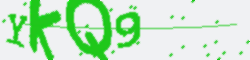
\includegraphics[width=1\linewidth]{imgs/textcaptcha/YKQ9.png}} 
        \\ а)
    \end{minipage}
    \begin{minipage}[h]{0.45\linewidth}
        \center{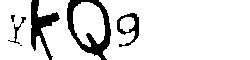
\includegraphics[width=1\linewidth]{imgs/textcaptcha/out.png}} 
        \\ б)
    \end{minipage}
    \caption{Изображения CAPTCHA: а) -- сгенерированное изображение, б) -- 
    результат обработки.}
    \label{fig:example-captcha}
\end{figure}

\vspace{-0.7cm}

\textbf{Подготовка датасета для CAPTCHA с изображениями}

Большинство предобученных моделей компьютерного зрения, таких как YOLOv8, обучены 
на датасете COCO~\cite{COCO}, содержащем изображения высокого качества с чёткими 
контурами и однозначной аннотацией объектов. Однако CAPTCHA с изображениями имеют 
принципиально иные характеристики: они могут включать в себя размытие, наложенные 
артефакты, искажения, шумы, повторяющиеся элементы и искусственно пониженное 
разрешение. Всё это снижает эффективность использования стандартных датасетов и 
моделей, не адаптированных под такие условия.

Для обеспечения высокой точности в задаче автоматического решения CAPTCHA 
необходимо подготовить собственный набор данных, приближённый к реальным условиям 
использования. Наиболее эффективным методом является автоматизированный парсинг 
изображений CAPTCHA, представленных на веб-сайтах, использующих визуальные 
CAPTCHA-решения, такие как Google reCAPTCHA v2.

Использование реальных CAPTCHA, собранных в автоматическом режиме, имеет ряд 
преимуществ по сравнению с синтетической генерацией данных:

\begin{enumerate}
    \item изображения содержат разнообразные сцены, освещение, углы обзора и 
    уровни шума, что положительно влияет на способность модели к обобщению;
    \item присутствует большое количество уникальных объектов на фоне, в том 
    числе в частично перекрытых и смазанных вариантах;
    \item отсутствует необходимость в ручной генерации изображений и создании 
    дополнительных искажений для повышения реалистичности;
    \item возможно извлекать текстовые инструкции к CAPTCHA, что позволяет 
    соотносить каждое изображение с требуемым классом.
\end{enumerate}

Для парсинга CAPTCHA был реализован автоматизированный сценарий взаимодействия с 
браузером с использованием библиотеки Selenium~\cite{Selenium}. Данный подход 
позволяет воспроизвести действия пользователя при работе с CAPTCHA, обходя при 
этом ручной ввод. Для обеспечения стабильной работы и масштабируемости процесса 
применялась браузерная автоматизация через WebDriver (в частности, ChromeDriver).

Функциональность парсера включает следующие ключевые этапы:

\begin{enumerate}
    \item поиск iframe-элемента, содержащего чекбокс <<Я не робот>>, и эмуляция 
    клика по нему для инициирования визуальной CAPTCHA;
    \item ожидание загрузки CAPTCHA и извлечение изображения с заданием (включая 
    его URL или пиксельный снимок);
    \item извлечение информации о структуре сетки (количество строк и столбцов), 
    на которую разбито изображение CAPTCHA;
    \item получение текста задания, содержащего имя объекта (например, <<выберите 
    все изображения с мотоциклами>>), для последующего использования в аннотации 
    данных.
\end{enumerate}

Типичная CAPTCHA представляет собой изображение, разделённое на сетку из 3×3 или 
4×4 ячеек, каждая из которых может содержать фрагмент сцены. При этом 
пользователю предлагается выбрать ячейки, в которых присутствует объект заданного 
класса. Процесс парсинга может быть представлена блок-схемой на рис.~
\ref{fig:captcha-flow}.

\begin{figure}[H]
    \centering
    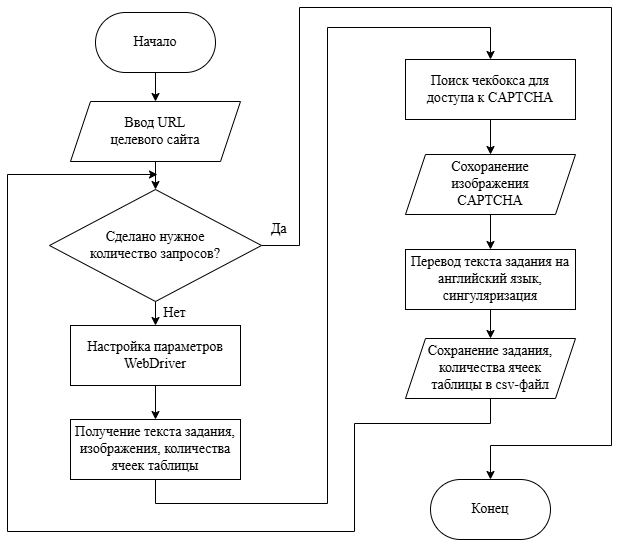
\includegraphics[width=0.6\textwidth]{
        imgs/imagecaptcha/image_captcha_flow.png
    }
    \caption{Блок-схема процесса парсинга CAPTCHA.}
    \label{fig:captcha-flow}
\end{figure}
\vspace{-0.5cm}

Полученные изображения и метаданные (включая текст задания и параметры сетки) 
используются для формирования обучающего датасета, пригодного для дообучения 
модели YOLOv8 в задачах классификации и сегментации объектов.

После получения достаточного количества изображений для составления датасета 
необходимо провести их предварительную обработку и разметку. Это один из 
самыхважных этапов работы, поскольку от качества разметки напрямую зависит 
точность и эффективность последующей работы модели.

Для корректной работы модели YOLO требуется создать иерархическую структуру 
папок, в которой изображения и соответствующие метки будут разделены на 
тренировочную и валидационную выборки. Стандартная структура включает следующие 
директории:

\begin{enumerate}
    \item Директория train -- содержит тренировочную выборку:
    \begin{enumerate}
        \item images -- изображения;
        \item labels -- метки к изображениям.
    \end{enumerate}
    \item Директория val -- содержит валидационную выборку:
    \begin{enumerate}
        \item images -- изображения;
        \item labels -- метки к изображениям.
    \end{enumerate}
\end{enumerate}

Набор классов, пути к выборкам и параметры конфигурации задаются в YAML-файле, 
который передается при обучении модели. Содержимое такого файла для данной 
модели:

\begin{code}
    \captionof{listing}{
        \label{code:train-captcha}Параметры конфигурации для обучения модели
    }
    \vspace{-0.75cm}
    {\small
        \inputminted[mathescape,linenos,frame=lines,breaklines]{yaml}{code/imagecaptcha/train_captcha.yaml}
    }
\end{code}
\vspace{-0.4cm}

Для создания меток используется инструмент CVAT (Computer Vision Annotation Tool) 
-- многофункциональное веб-приложение с поддержкой аннотации объектов с помощью 
полигонов, прямоугольников и других форм. CVAT позволяет экспортировать разметку 
напрямую в формат, совместимый с YOLO~\cite{CVAT}.

Поскольку CAPTCHA-изображения часто содержат объекты с нечёткими контурами, 
наложением и визуальными искажениями, особенно важно использовать ручную точную 
разметку, а не ограничиваться автоматическими методами. Выделение объектов должно 
проводиться как можно точнее, с учётом геометрии контуров. На рисунке ниже 
представлен пример изображения с размеченными объектами:

\begin{figure}[H]
    \centering
    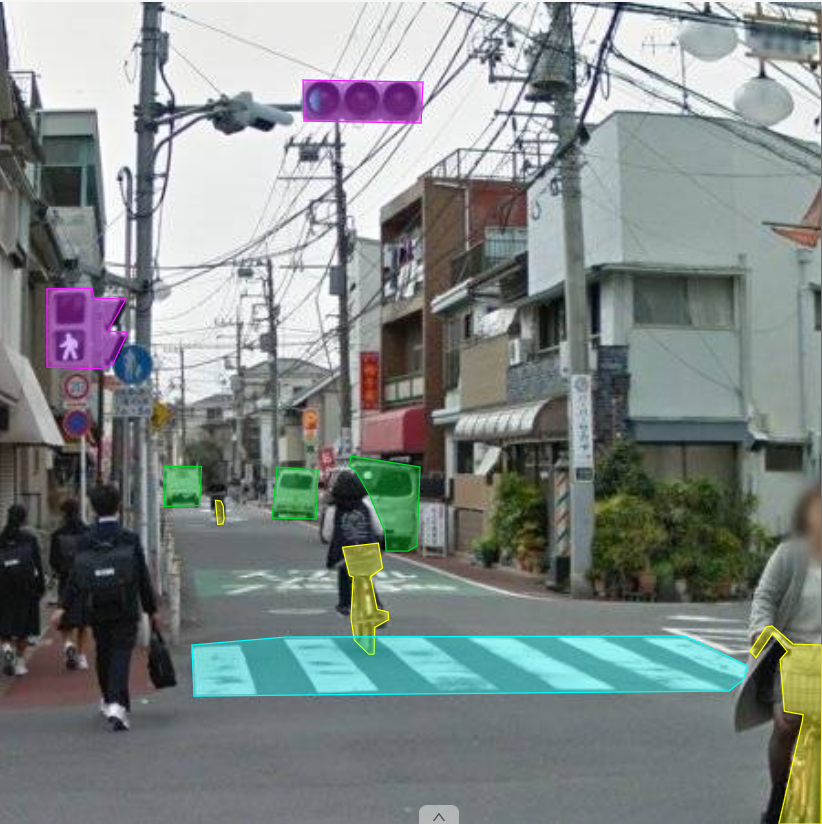
\includegraphics[width=0.9\linewidth]{imgs/imagecaptcha/captcha-poligons.png}
    \caption{Пример разметки изображения с тестовой CAPTCHA.}
    \label{fig:mask-captcha}
\end{figure}
\vspace{-0.5cm}

Кроме того, разметка позволяет учесть сразу несколько объектов разных классов на 
одном изображении, что особенно характерно для CAPTCHA, где в одной сетке могут 
одновременно находиться, например, автомобили и автобусы. Такой подход 
положительно влияет на обобщающую способность модели.

В случае, если количество данных по отдельным классам окажется недостаточным, 
можно дополнительно использовать методы аугментации: вращение, масштабирование, 
искажение цвета и контраста. Однако при хорошо организованном парсинге и разметке 
зачастую удается обойтись без аугментации.
